\documentclass[
  french,
  a4paper,
]{scrartcl}

\usepackage[pages=some]{background}
%\usepackage{subfigure}
\usepackage{subcaption}
% \backgroundsetup{firstpage = true, scale = 1, angle = 0, opacity = 1, 
% contents = {\includegraphics[width = \paperwidth, height = \paperheight] {arc-template.pdf}}}
\usepackage{listings}
\usepackage{siunitx}
\usepackage[most]{tcolorbox}
\usepackage{xcolor}
\definecolor{codegreen}{rgb}{0,0.6,0}
\definecolor{codegray}{rgb}{0.5,0.5,0.5}
\definecolor{codepurple}{rgb}{0.58,0,0.82}
\definecolor{backcolour}{rgb}{0.98,0.98,0.98}

\lstdefinestyle{mystyle}{
    backgroundcolor=\color{backcolour},   
    commentstyle=\color{codegreen},
    keywordstyle=\color{magenta},
    numberstyle=\tiny\color{codegray},
    stringstyle=\color{codepurple},
    basicstyle=\ttfamily\normalsize,
    breakatwhitespace=false,         
    breaklines=true,                 
    captionpos=b,                    
    keepspaces=true,                 
    numbers=left,                    
    numbersep=5pt,                  
    showspaces=false,                
    showstringspaces=false,
    showtabs=false,                  
    tabsize=2
}
\lstset{style=mystyle}

\usepackage{amsmath,amssymb}
\usepackage[french]{babel}

\usepackage[T1]{fontenc}
\usepackage[utf8]{inputenc}
\usepackage{graphicx}
\usepackage{tabularx}

\usepackage{lmodern}

\usepackage[
  top=2cm, 
  bottom=3.5cm, 
  left=2cm, 
  right=2cm,
  includefoot
  ]{geometry}
\usepackage[hidelinks]{hyperref}

\renewcommand{\arraystretch}{1.2}
\setlength {\parindent}{0em}
\setlength {\parskip}{1em}

\usepackage{scrlayer-scrpage}

\setkomafont{author}{\sffamily}
\setkomafont{date}{\sffamily}
\setkomafont{subject}{\sffamily}

\addtokomafont{title}{\raggedright}
\addtokomafont{author}{\raggedright}
\addtokomafont{date}{\raggedright}

%\setkomafont{section}{\normalfont\Large\bfseries\rmfamily}
%\setkomafont{subsection}{\normalfont\large\bfseries\rmfamily}
%\setkomafont{subsubsection}{\normalfont\normalsize\bfseries\rmfamily}

\setlength{\headsep}{0.5cm}
\setlength{\headheight}{2cm}

\makeatletter
\renewcommand*\maketitle{
    \sffamily
    \Large 3293.3 JEE/Spring II $\cdot$ 2023-2024 $\cdot$ ISC3il-a

    \huge \textbf{NeoLib - Un système de gestion de bibliothèque}
    \vspace{10pt}
    \Large\rmfamily
    
    Nima Dekhli\\
    
    \vspace{8pt}
    %\large Projet n°264 \hfill Version 1.0 \hfill \today
    \large
    \today

}
\makeatother

% setup header on title page
%\clearpairofpagestyles

\newpairofpagestyles{firstpage}{
   \ihead{
    \includegraphics*[height=1.5cm]{img/he-arc.png}
  }
  \ohead{
       \includegraphics*[height=1.0cm]{img/hes-so.png}
  } 
  \cfoot{\pagemark}
}

\begin{document}
\thispagestyle{firstpage}
\maketitle
\tableofcontents
\newpage
 
\section{Introduction}

\subsection{Contexte}

Dans le cadre du cours de JEE/Spring II, il nous est demandé d'implémenter une API 
qui utilise le pattern \textit{microservices}. Le sujet du projet est libre, tant qu'il 
respecte les contraintes minimales. 


\subsection{Choix du sujet}

NeoLib est un système de gestion des bibliothèques. Il permet de gérer les livres à disposition 
et les emprunts des utilisateurs. 


\section{Architecture implémentée}

Deux services distincts coexistent et se complètent. Le premier service, \textit{book-service}, 
permet la gestion des livres, avec toutes les méta-données qui les composent. Le second service,
\textit{loan-service}, permet la gestion des emprunts par les utilisateurs. 

Chacun des services possède sa propre base de données. Le service \textit{loan-service} est
dépendant du service \textit{book-service} pour la gestion des emprunts. En effet, un emprunt
ne peut être effectué que si le livre existe et est disponible. Il doit donc effectuer 
une requêtes synchrone pour interroger le service \textit{book-service}. 

Les communications synchrones sont effectuées en utilisant le protocole HTTP. Les communications
asynchrones sont effectuées en utilisant le protocole AMQP. Afin d'effectuer du \textit{load balancing},
une gateway est utilisée pour rediriger les requêtes vers les services. Tous les services 
s'enregistrent auprès du registre Eureka.

Sur la figure \ref{fig:architecture}, on peut voir l'architecture générale du système.

\begin{figure}[h]
    \centering
    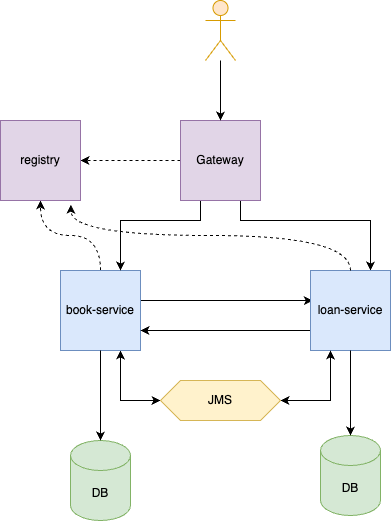
\includegraphics[width=0.8\textwidth]{img/neolib.png}
    \caption{Architecture générale du système}
    \label{fig:architecture}
\end{figure}

\subsection{book-service}

Ce service est une simple base de données de livres. L'API permet de lister les livres,
d'en ajouter, d'en supprimer et de les modifier. Les champs suivants sont disponibles pour
chaque livre:

\begin{itemize}
    \item ID (généré automatiquement)
    \item ISBN
    \item Titre
    \item Auteur
    \item Statut
\end{itemize}

Le statut permet de savoir si le livre est disponible, emprunté, perdu ou bloqué. 


\subsection{loan-service}

Ce service permet la gestion des emprunts ainsi que des utilisateurs. 
Un utilisateur doit exister dans la base de données pour pouvoir emprunter un livre. 

L'API permet d'emprunter un livre, de le rendre, de lister les emprunts en cours (pour un utilisateur donné)
et de savoir qui a emprunté un livre donné. De plus, il est possible de marquer un livre comme perdu. 


\section{Flux de communications entre les services}

\subsection{Flux de communication synchrones}

Les flux de communication synchrones sont effectués en utilisant le protocole HTTP. Ils sont 
uniquement utilisés pour effectuer des requêtes depuis le service \textit{loan-service} vers le service
\textit{book-service}. 

Il y a deux cas d'utilisation des communications synchrones:

\begin{itemize}
  \item Lors de l'emprunt d'un livre, le service \textit{loan-service} doit récupérer 
    les informations du livre (méta-données) pour compléter sa base de données locale et pour 
    vérifier que le livre est bien disponible ; 

  \item Lors de la perte d'un livre, le service \textit{loan-service} doit marquer le livre
    comme perdu dans la base de données du service \textit{book-service}.
\end{itemize}

Afin d'effectuer du \textit{client-side load balancing}, on utilise un client Feign pour effectuer
les requêtes HTTP.

\subsection{Flux de communication asynchrones}

\section{Guide de démarrage}

\section{Conclusion}
 
\end{document}
